\chapter{实验结果及分析}
\label{chap:experiment}

在此部分,本文将首先全方位检验提出的用于创新3D药物分子设计的几何促进的分子扩散框架GFMDiff在生成3D分子任务中的表现,用于性能比较的三个任务和两个公开数据集都具备极强的代表性。同时为了进一步探究本文提出的DTN去噪内核作为分子学习模型,在分子性质预测任务上的表现。本文将DTN与时下性能最优的3D分子学习模型,在2个公开数据集上的表现进行对比。

\section{药物分子设计}
在本节中,我们报告了GFMDiff在两个主流数据集GEOM-QM9 \cite{qm9_ramakrishnan_14}和GEOM-Drugs \cite{drugs_axelrod_22}上的三个生成任务中的表现。本文采用了时下最前沿的相关研究模型作为基线模型,在采取一致的实验条件的前提下,直接引用他们生成的实验结果。结果表明,我们的方法在多个方面显著优于该领域最优秀的模型,展现出在3D分子生成任务中时下最优的性能。

\subsection{实验设置}

\textbf{数据集:}
为了进行全面且公平的比较,我们在两个基准数据集(GEOM-QM9和GEOM-Drugs)上进行了三组实验:在GEOM-QM9上的药物分子设计,在GEOM-QM9上有条件的药物分子设计,和在GEOM-Drugs上的药物分子设计。具体的数据集处理工作较为琐碎,本文将在对应的生成任务实验分析中分别介绍。

GEOM-QM9数据集(简称:QM9)是一个广泛运用在基于深度学习的分子学习领域的数据集,包含超过13万个分子及其对应的构象,以及每个分子对应的19种性质。数据集中,在包含氢原子条件下,平均每个分子有19个原子,其中最大的分子有29个原子。同时,整个数据集的分子仅包括氢,碳,氮,氧,氟这五种原子。

GEOM-Drugs(简称:Drugs)是一个规模相对更大的数据集,其包括的分子数量和每个分子所含平均原子数都较多。该数据集记录了超过45万个分子和它们对应的3700万个不同构象。在包含氢原子的条件下,平均每个分子由44个原子构成,最大的由181个原子构成。同时,整个数据集的分子包含16类原子,较QM9比原子种类更丰富。

\textbf{评价指标:}
为公平的评价GFMDiff的性能并与时下最优秀的模型对比,本文采用目前该领域通用的评价指标,具体介绍如下。

$\bullet$ 负对数似然函数(Negative log-likelihood / NLL):是一个被广泛应用于评价参数估计的指标,其在深度学习中也可以被用作损失函数。

$\bullet$ 稳定性(Stability):是3D分子设计领域最重要的评价指标,其衡量了生成的分子构型和化学键在几何空间内是否稳定。对于一个化学键而言,根据其两端连接的原子的类型和化学键类型的不同,在计算化学上存在不同的理想稳定键长\footnote{\url{http://www.wiredchemist.com/chemistry/data/bond_energies_lengths.html}}\footnote{\url{https://www.mrbigler.com/documents/Chemistry_Reference_Tables.pdf}}。例如对两个碳原子,其可能形成单键,双键和三键。对于碳碳单键,双键和三键,其理论键能分别为346,602,835(千焦/摩尔),对应键长分别为154,134,120(皮米)。对于模型生成的分子几何构象,若一对碳原子间距离小于120皮米,则认为这两个碳原子由三键连接,若距离大于120皮米,且小于134皮米,则认为它们由双键连接。若原子间距离超过154皮米,则认为两者之间不存在键相连。根据计算化学相关知识,若一个原子经过预测,连接的所有键总计化合价预期理论值一致,则认为该原子稳定。以碳原子为例,若其经过预测后与4个其他原子形成单键,或形成2个单键1个双键,则认为该碳原子是稳定的。如果一个分子中所有的原子都具备正确的化合价,则该分子也被认为是稳定的。该指标有效的同时衡量生成的三维分子构象的几何和拓扑性质。在具体评价中,稳定性可分为原子稳定性(Atom Stability)和分子稳定性(Molecule Stability),他们各自代表稳定原子/分子在所有原子/分子中的数量占比。

$\bullet$ 有效性(Validity):是在2D和3D分子生成领域通用的评价指标,其衡量了有效分子在所有分子中的数量占比。 一个分子的有效与否,决定于RDKit中对分子中化合价和度的判断。

$\bullet$ 唯一性(Uniqueness):同样对2D和3D分子设计通用,该指标衡量了生成结果中非重复的分子的数量占比。

$\bullet$ 平均绝对误差(Mean absolute error / MAE):是一个常用于回归任务的评价指标。在本文中,该指标仅用于评价有条件的分子生成的样本属性。

\textbf{基线模型:}
本文采用了本领域最具代表性且最前沿的模型,包含基于自回归模型的,流型模型的和扩散模型的方法。

$\bullet$ E-NF\cite{enf_satorras_21}是基于流型模型的3D分子设计的模型。其中用于图学习的网络为等变的EGNNs\cite{egnn_satorras_21}。该网络将原子间距离视作键的特征,通过信息传递更新相应节点特征。

$\bullet$ G-SchNet\cite{gschnet_wallach_19}在SchNet\cite{schnet_schutt_17}的基础上设计了一个自回归模型,通过逐步生成原子和键的方式生成分子结构。SchNet已经被证明其对角度信息具备良好提取能力。

$\bullet$ EDM\cite{edm_hoogeboom_22}是最早将扩散模型引入到药物分子设计的模型。其去噪内核同样采用EGNNs\cite{egnn_satorras_21}。

$\bullet$ Bridge和Bridge+Force\cite{diffpg_wu_22}提出能量方式用于更有效的引入几何信息,通过分子间作用力,引导分子生成更有效更稳定的构型。

$\bullet$ GCDM\cite{gcdm_morehead_23}是距今该领域表现最好且拥有完整开源代码的方法。其参照ColfNet的思路\cite{colfnet_du_22}引入了完整的空间几何信息。

为了公平客观的评价GFMDiff的性能,本文选取的基线模型都是具备完整可复现开源代码的模型,并在采用一致基本参数设置的条件进行实验。本文引用了EDM\footnote{\url{https://github.com/ehoogeboom/e3_diffusion_for_molecules}}实验部分中E-NF,G-SchNet和EDM的表现,引用了Bridge和Bridge+Force的实验结果,以及GCDM\footnote{\url{https://github.com/BioinfoMachineLearning/bio-diffusion}}的实验结果。

\textbf{实验环境:}
本文在生成实验上基于的硬件平台如下:

GEOM-QM9实验:Intel(R) Xeon(R) Platinum 8358和2 * NVIDIA A100 SXM4 40GB; 

GEOM-Drugs实验: AMD EPYC 7742和4 * NVIDIA A100 PCIe 80GB。

此外,相关实验依赖的一些重要的包有:CUDA 11.4,Python 3.9.13,PyTorch 1.10.0,PyG 2.0.4,RDKit 2022.03.5。

\subsection{在GEOM-QM9上的药物分子设计}
\begin{table}[h]
    \centering
    \caption{GEOM-QM9上药物分子设计结果对比}
    \label{tab:gen_qm9}
    \begin{tabular}{lllllll}
    \toprule
    Type & Method & NLL$\downarrow$ & \makecell[l]{Atom\\Stability\\(\%) $\uparrow$} & \makecell[l]{Mol\\Stability\\(\%) $\uparrow$} & \makecell[l]{Validity\\(\%) $\uparrow$} & \makecell[c]{Uniqueness\\$\times$\\Validity(\%) $\uparrow$} \\
    \midrule
    NF & E-NF & -59.7 & 85.0 & 4.9 & 40.2 & 39.4 \\
    \cline{2-7}
    AR & G-SchNet & N/A & 95.7 & 68.1 & 85.5 & 80.3 \\
    \cline{2-7}
    \multirow{2}{*}{DDPM}
    & EDM & -110.7$\pm$1.5 & 98.7$\pm$0.1 & 82.0$\pm$0.4 & 91.9$\pm$0.5 & 90.7$\pm$0.6 \\
    & Bridge & N/A & 98.7$\pm$0.1 & 81.8$\pm$0.2 & N/A & N/A \\
    & Bridge+Force & N/A & \underline{98.8}$\pm$0.1 & 84.6$\pm$0.3 & N/A & N/A \\
    & GCDM & \textbf{-171.0}$\pm$0.2 & 98.7$\pm$0.0 & 85.7$\pm$0.4 & 94.8$\pm$0.2 & 93.3$\pm$0.0 \\
    \midrule
    \multirow{2}{*}{\makecell[l]{DDPM\\(Ours)}} & \makecell[l]{GFMDiff\\w/o tri} & -123.1$\pm$0.4 & 98.7$\pm$0.1 & 85.9$\pm$0.2 & 94.9$\pm$0.2 & 94.2$\pm$0.2 \\
    & \makecell[l]{GFMDiff\\w/o GFLoss} & -127.5$\pm$0.4 & 98.7$\pm$0.0 & \underline{87.5}$\pm$0.1 & \underline{96.0}$\pm$0.0 & \underline{95.2}$\pm$0.0 \\
    & GFMDiff & \underline{-132.5}$\pm$0.2 & \textbf{99.1}$\pm$0.0 & \textbf{91.3}$\pm$0.2 & \textbf{97.0}$\pm$0.3 & \textbf{96.1}$\pm$0.2 \\
    \midrule
    Data &  &  & 99.0 & 95.2 & 97.7 & 97.7 \\
    \bottomrule
    \end{tabular}
\end{table}
\begin{figure}[h]
    \centering
    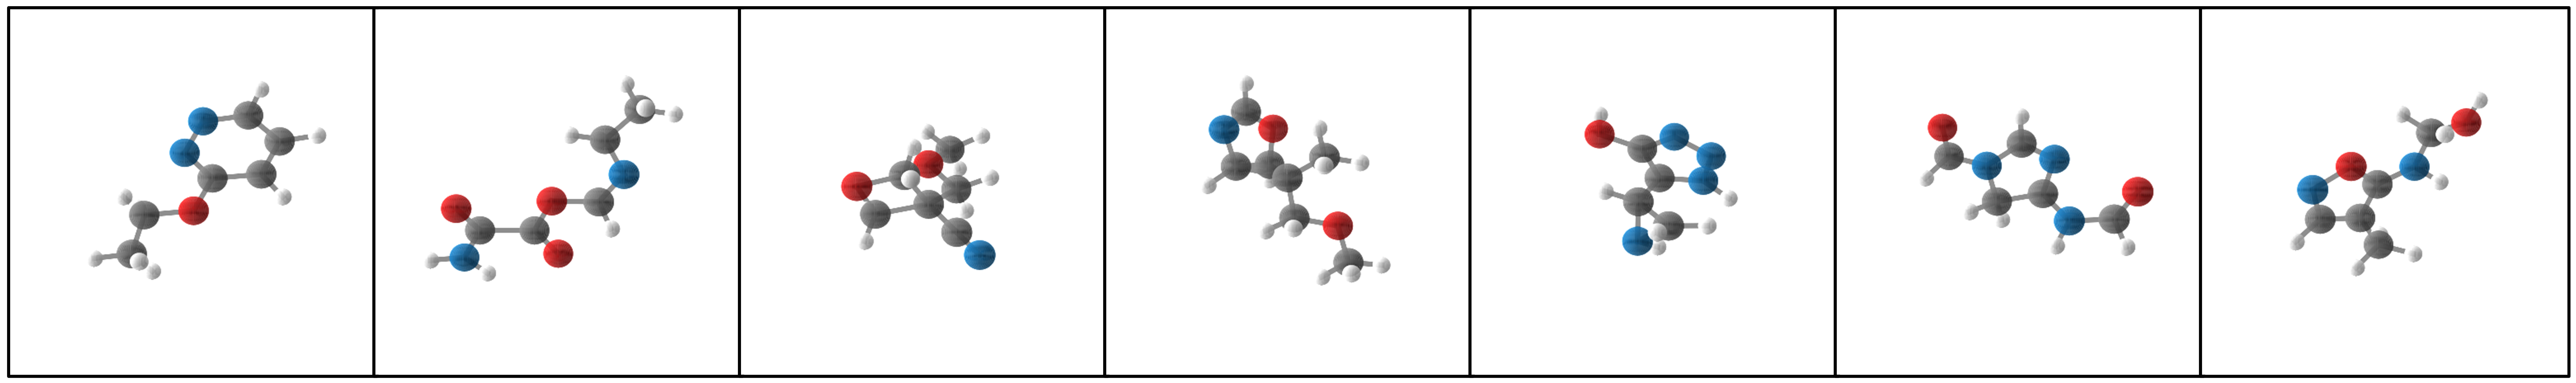
\includegraphics[width=\linewidth]{figures/samples_qm9.png}
    \caption{GFMDiff在GEOM-QM9上药物分子设计样本示意}
    \label{fig:samples_qm9}
\end{figure}

在该任务的实验中,本文依照先前研究,将QM9数据集分别划分为样本大小为10万,1.8万和1.3万的训练集,验证集和测试集。表~\ref{tab:gen_qm9}~为GFMDiff和基线模型在分子在QM9数据集上的表现对比,指标旁的箭头代表更优取值的方向。同时图~\ref{fig:samples_qm9}~展示了部分生成分子的三维构象。NLL的取值为模型在测试集上的得分,而剩余指标的计算基于模型随机生成的10000个样本。此外,部分基线模型的特定指标可能在先前研究没有说明,在此用N/A替代。在表中,最好和次好的结果分别以粗体和下划线的形式予以强调。

除了在测试集上的NLL得分,本文在其他的所有指标上都显著优于基线模型。稳定性作为创新3D药物分子设计任务中的核心指标,GFMDiff在这两个评价指标中较先前研究有明显优势,分子稳定性较表现最好的基线模型有6.5\%的提升,这证明了GFMDiff对几何信息的有效利用极大的提升了模型性能。在有效性层面,GFMDiff较表现最好的基线模型的提升分别为2.3\%和3\%。这说明了GFMDiff能够生成有效且非重复的分子。值得一提的是,GFMDiff生成结果已经十分接近,甚至在个别指标上超过了数据本身,实验结果充分表明了本文提出的GFMDiff在生成中型分子时具备的优异性能。

为衡量本文提出的的DTN去噪内核和GFLoss损失函数的有效性,本文进行了两组消融实验。在此,将GFLoss损失函数的权重$\lambda$设置为0,则可以得到GFMDiff w/o GFLoss模型。在此基础上,本文将DTN中原子对-三元组间的注意力机制模块取代为一个原子对自注意力机制模块,得到GFMDiff w/o tri模型。GFMDiff w/o GFLoss消融实验的结果表明本文引入的GFLoss损失函数对生成稳定、有效的药物分子三维构象有积极促进作用。其在评价指标上全面落后于GFMDiff。GFMDiff w/o tri模型的结果较另外两个GFMDiff模型有更大的降幅。这样的结果表明DTN中对分子三元组信息的提取,并将其融入原子对距离学习是有效的。作为表现最差的GFMDiff模型变体,该模型仍优于其他基线模型,这也足以说明双轨Transformer网络中的双轨设计和基于Transformer的分子图学习的有效性。

\subsection{在GEOM-QM9上有条件的药物分子设计}
除了最基本的稳定性和有效性,生成具备良好属性的药物分子是药物分子生成模型应当具备的一项能力。为评价模型在有条件的药物分子生成任务上的表现,本文根据通行做法开展实验。在QM9数据集包含的所有性质中,选取各向同性极化率$\alpha$,最高占据分子轨道$\varepsilon_{{\rm HOMO}}$,最低未占分子轨道$\varepsilon_{{\rm LUMO}}$,两者间能量隙$\Delta \varepsilon$,偶极矩$\mu$和298.15K时的热容$C_v$。

\begin{table}[h]
    \centering
    \caption{GEOM-QM9上有条件的药物分子设计结果对比}
    \label{tab:gen_qm9_condition}
    \begin{tabular}{lllllll}
    \toprule
    \makecell[l]{Task\\Units} & \makecell[l]{$\alpha$\\${\rm Bohr^3}$} & \makecell[l]{$\Delta \varepsilon$\\${\rm meV}$} & \makecell[l]{$\varepsilon_{{\rm HOMO}}$\\${\rm meV}$} & \makecell[l]{$\varepsilon_{{\rm LUMO}}$\\${\rm meV}$} & \makecell[l]{$\mu$\\${\rm D}$} & \makecell[l]{$C_v$\\$\frac{{\rm cal}}{{\rm mol}}{\rm K}$} \\
    \midrule
    Naive (Upper-bound) & 9.01 & 1470 & 645 & 1457 & 1.616 & 6.857 \\
    \# Atom & 3.86 & 866 & 426 & 813 & 1.053 & 1.971 \\
    EDM & 2.76 & 655 & 356 & 584 & 1.111 & 1.101 \\
    GCDM & \underline{1.97} & \underline{602} & \underline{344} & \underline{479} & \underline{0.844} & \underline{0.689} \\
    GFMDiff & \textbf{1.74} & \textbf{558} & \textbf{321} & \textbf{430} & \textbf{0.728} & \textbf{0.593} \\
    QM9 (Lower-bound) & 0.10 & 64 & 39 & 36 & 0.043 & 0.040 \\
    \bottomrule
    \end{tabular}
\end{table}

\begin{figure}[h]
    \centering
    \includegraphics[width=\linewidth]{figures/samples_qm9_cond.png}
    \caption{GFMDiff在GEOM-QM9上有条件的药物分子设计样本示意}
    \label{fig:samples_qm9_cond}
\end{figure}

为检验生成的药物分子是否具备良好属性,在实验时,需要将QM9数据集的训练集部分平均分为两部分。在训练阶段,第一部分被用作一个EGNN\cite{egnn_satorras_21}神经网络的训练。该网络通过学习正确的分子及对应的属性,故将具备根据输入分子预测相应性质的能力。第二部分数据集被用作生成模型的训练,即在普通的生成模型基础上,在训练时增加对应性质信息。在两部分都完成训练后,则预先根据训练集中性质的均值和方差,采样得到需要生成样本具备的性质。根据这部分性质,生成模型会生成10000个采样结果。这部分采样结果将通过之前训练好的EGNN神经网络,进行对应的性质预测,最终的衡量标准为EGNN预测的分子性质和分子生成时依照的性质间的平均绝对误差。

在基线模型上,本文引入了三个参照模型:Naive,\#Atom和QM9。Naive模型在测试阶段时,EGNN模型根据随机打乱原有的采样样本对应性质并预测相应结果,这代表了在此任务下预测结果MAE的取值上限。\#Atom模型在测试阶段,EGNN模型仅依据分子所含原子数对性质进行预测。如果生成模型的测试MAE较\#Atom模型低,则说明该模型能够根据特定性质生成相应的分子。参照模型QM9则代表EGNN在QM9数据集上的预测性能,该表现代表分子性质预测结果的MAE下界。

根据表~\ref{tab:gen_qm9_condition}~所示,本文提出的GFMDiff在测试任务中预测结果的MAE均低于目前最优的GCDM模型,在所有六个指标中的领先幅度分别为:11.7\%,7.3\%,6.7\%,10.2\%和13.7\%。该表现足以证明,GFMDiff具备根据指定条件生成分子的能力。图~\ref{fig:samples_qm9_cond}~中全面的展示了GFMDiff依据不同的性质取值,生成对应的药物分子样本。以各向同性极化率$\alpha$为例,随着$\alpha$取值增加,模型倾向于生成更长的碳链。

\subsection{在GEOM-Drugs上的药物分子设计}
在GEOM-Drugs数据集基础上进行创新药物分子设计是一个具有挑战性的任务,因为该数据集不仅包含分子多,也因其中分子主要为大分子,这对分子图中键的形成提出了较高的要求。在对GEOM-Drugs的实验中,我们将GFMDiff与E-NF、EDM、Bridge+Force和GCDM进行了比较。此外,由于当前方法面对如此庞大且自身数据不够精良的生成任务时,较QM9数据集上的表现有较大差距,常常无法生成新的分子,故在此讨论生成分子的有效性是缺乏意义的。在评价指标方面,本文采用了生成10000个药物分子的稳定性用作性能比较。

\begin{table}[h]
    \centering
    \caption{GEOM-Drugs上药物分子设计结果对比}
    \label{tab:gen_drugs}
    \begin{tabular}{llll}
    \toprule
    Type & Method & Atom Stability (\%) $\uparrow$ & Mol Stability (\%) $\uparrow$ \\
    \midrule
    Normalizing flow & E-NF & 75.0 & 0 \\
    \multirow{2}{*}{DDPM}
    & EDM  & 81.3 & 0.0 \\
    & Bridge & 81.0$\pm$0.7 & 0.0 \\
    & Bridge+Force & 82.4$\pm$0.8 & 0.0 \\
    & GCDM & 86.4$\pm$0.2 & 3.7$\pm$0.3 \\
    \midrule
    Ours & GFMDiff & \textbf{86.5}$\pm$0.2 & \textbf{3.9}$\pm$0.2 \\
    \midrule
    Data &  & 86.5 & 2.8 \\
    \bottomrule
    \end{tabular}
\end{table}
\begin{figure}[h]
    \centering
    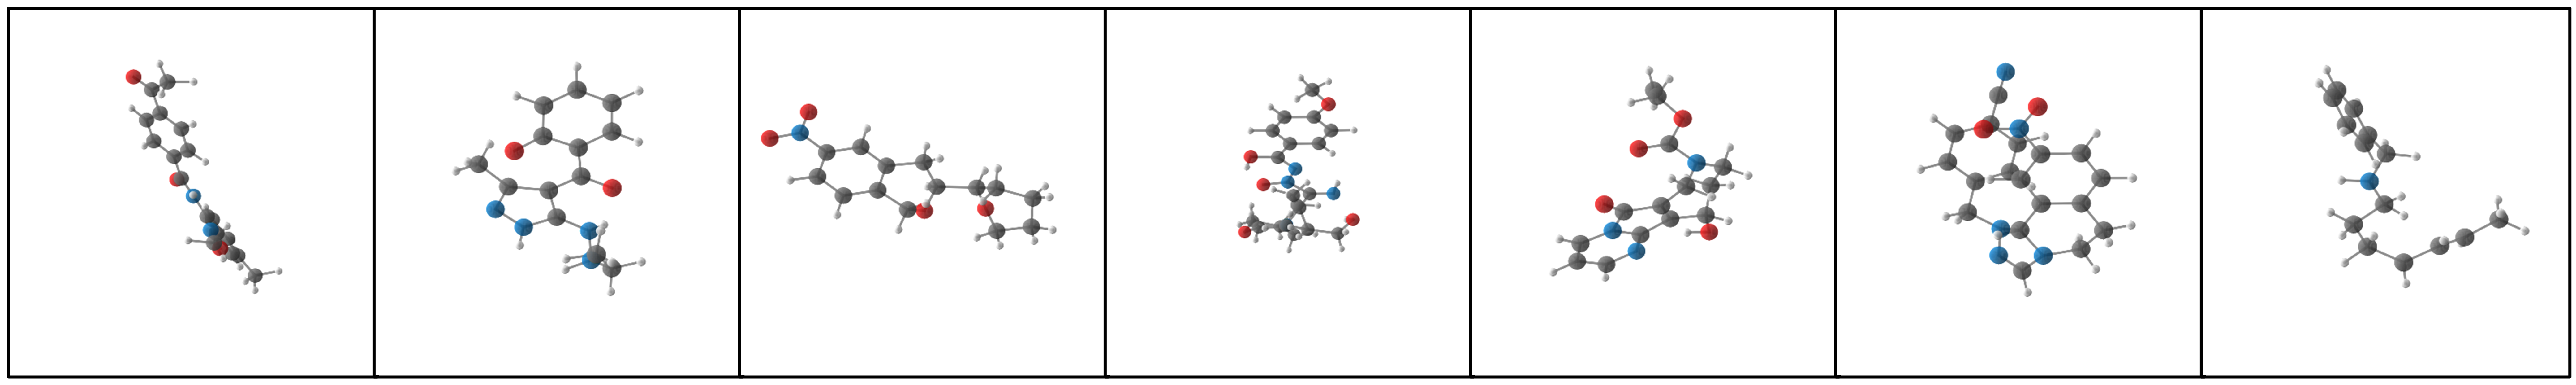
\includegraphics[width=\linewidth]{figures/samples_drugs.png}
    \caption{GFMDiff在GEOM-Drugs上药物分子设计样本示意}
    \label{fig:samples_drugs}
\end{figure}

由于GEOM-Drugs中分子庞大,且该数据集不如QM9精确,其自身的稳定性就比QM9中要低得多。由表~\ref{tab:gen_drugs}~与QM9上实验展现出的优秀表现一致,本文提出的GFMDiff在原子稳定性方面略优于GCDM,同时显著优于其他基线模型。在分子的整体稳定性方面,GFMDiff的表现超过第二名结果5.4\%。图~\ref{fig:samples_drugs}~展示了部分生成分子的三维构象。在Drugs上的结果也足以证明了本文提出的GFMDiff在捕捉三维原子相互作用并生成的分子键时的强大能力。


\section{分子性质预测}
在AI辅助药物发现领域,分子性质预测也是十分基础的研究问题。为验证本文提出的双轨Transformer网络(DTN)对三维分子几何信息的学习能力,本文在两个大型公开分子数据集上进行了全面的实验。

\subsection{实验设置}
\textbf{数据集:}在分子性质预测实验中,本文使用了两个广泛使用的基准公开数据集:OC20和GEOM-QM9。在此,本节只介绍OC20数据集的详细信息。

$\bullet$ Open Catalyst 2020 (OC20) \cite{oc20_chanussot_21}数据集是一个较新的公开大规模数据集,用于建模和发现催化剂。具体而言,其目标是对结构弛豫进行高效的密度泛函理论(Density functional theory / DFT)近似计算。在催化剂研究中,结构弛豫是一项基础计算任务,其被用于确定结构的活性和选择性。数据集中的所有结构都包含一个表面和一个吸附物,表面由一个周期性的晶胞定义。该数据集中包括三个任务,分别是结构到能量和力(S2EF),初始结构到弛豫结构(IS2RS)和初始结构到弛豫能量(IS2RE)。本文中,我们聚焦于初始结构到弛豫能量(IS2RE)任务,这是催化剂研究中最常见的任务,因为弛豫能量通常与催化剂的活性和选择性相关。与相关研究采取的设置类似,本文将IS2RE的数据集分为训练集、验证集和测试集。训练集包含460,328个分子结构,验证集分为域内(ID)、域外吸附物(OOD Ads)、域外催化剂(OOD Cat)和域外吸附物和催化剂(OOD Both)四个子集,分别包含24,733、24,961、24,738、24,971个结构。

\textbf{评价指标:}
在回归任务中,本文主要采取预测结果的MAE作为衡量评价模型预测准确程度的指标。此外在OC20的任务上,本文还引入了真实能量阈值内占比(Energies within a Threshold)作为另一衡量指标。

\textbf{基线模型:}
在基线模型的选择上,本文选取了时下最优的有可复现代码的模型用于性能对比。包括CGCNN \cite{cgcnn_xie_18},SchNet \cite{schnet_schutt_17},PhysNet \cite{physnet_unke_19},MGCN \cite{mgcn_lu_19},DimeNet++ \cite{dimenetpp_gasteiger_20},GemNet \cite{gemnet_gasteiger_21},PaiNN \cite{painn_schutt_21},SphereNet \cite{spherenet_liu_22}和ComENet \cite{comenet_wang_22}。

\subsection{在GEOM-QM9数据集上的分子性质预测}
为检测DTN在分子性质预测上的性能和在量子化学系统中的预测能力,我们将DTN应用于QM9数据集上的分子性质预测任务。表~\ref{tab:reg_qm9}~展示了本文DTN和基线模型在回归任务上结果的MAE对比,任务包括12种性质及所有任务上的总体均方根误差(std. MAE)。其中每项任务表现最佳和次佳的结果分别以粗体和下划线的形式予以强调。

\begin{table}[h]
    \begin{center}
    \caption{GEOM-QM9上药物分子性质预测结果对比}
    \label{tab:reg_qm9}
    \resizebox{\textwidth}{!}
    % \small
    {\begin{tabular}{llcccccccc}
    \toprule
    Property & Unit & SchNet & PhysNet & MGCN & DimeNet++ & PaiNN & SphereNet & ComENet & DTN \\
    \midrule
    $\mu$ & D & 0.033 & 0.0529 & 0.0560 & 0.0297 & \textbf{0.012} & 0.0245 & 0.0245 & \underline{0.0162} \\
    $\alpha$ & ${a_0}^3$ & 0.235 & 0.0615 & \underline{0.0300} & 0.0435 & 0.045 & 0.0449 & 0.0452 & \textbf{0.0279} \\
    $\varepsilon_\text{HOMO}$ & meV & 41 & 32.9 & 42.1 & 24.6 & 27.6 & \underline{22.8} & 23.1 & \textbf{20.7} \\
    $\varepsilon_\text{LUMO}$ & meV & 34 & 24.7 & 57.4 & 19.5 & 20.4 & \underline{18.9} & 19.8 & \textbf{16.6} \\
    $\Delta\epsilon$ & meV & 63 & 42.5 & 64.2 & 32.6 & 45.7 & \underline{31.1} & 32.4 & \textbf{28.8} \\
    $\left< R^2 \right>$ & ${a_0}^2$ & 0.073 & 0.765 & \underline{0.110} & 0.331 & \textbf{0.066} & 0.268 & 0.259 & 0.145 \\
    ZPVE & meV & 1.7 & 1.39 & \underline{1.12} & 1.21 & 1.28 & \underline{1.12} & 1.20 & \textbf{1.08} \\
    $U_0$ & meV & 14 & 8.15 & 12.9 & 6.32 & \underline{5.85} & 6.26 & 6.59 & \textbf{5.34} \\
    $U$ &meV    & 19 & 8.34 & 14.4 & 6.28 & \underline{5.83} & 6.36 & 6.82 & \textbf{5.46} \\
    $H$ &meV    & 14 & 8.42 & 14.6 & 6.53 & \underline{5.98} & 6.33 & 6.86 & \textbf{5.60} \\
    $G$ &meV    & 14 & 9.4 & 16.2 & 7.56 & \underline{7.35} & 7.78 & 7.98 & \textbf{6.69} \\
    $c_\text{v}$ & $\frac{\mbox{cal}}{\mbox{mol K}}$ & 0.033 & 0.028 & 0.038 & 0.023 & 0.024 & \underline{0.022} & 0.024 & \textbf{0.021} \\
    \midrule
    std. MAE & \% & 1.76 & 1.37 & 1.86 & 0.98 & 1.01 & \underline{0.91} & 0.93 & \textbf{0.089} \\
    \bottomrule
    \end{tabular}}
    \end{center}
    \vspace{-10 pt}
    \end{table}

DTN在11个性质预测任务上取得了最佳性能,并在1个性质预测任务上取得了次佳性能。同时DTN将QM9数据集的总体预测结果的均方根误差从0.91降低到0.89,实现更稳定的预测结果。实验结果说明了本文的DTN网络在分子图学习领域同样具备良好的性能。

\subsection{在OC20数据集上的分子性质预测}
Open Catalyst 2020(OC20)数据集\cite{oc20_chanussot_21}是一个新发布的大规模数据集,其被用于催化剂的发现和优化。该数据集包含了数百万个DFT弛豫计算结果,涵盖了巨大的化学结构空间,以便可以完全训练机器学习模型。

本研究专注于IS2RE任务。Chanussot等\cite{oc20_chanussot_21}的研究中的研究中提供了CGCNN、SchNet和DimeNet++的结果。原始的GemNet论文中没有其在OC20数据集的结果,故本文使用OC项目网站上公开可用的代码\footnote{\url{https://github.com/Open-Catalyst-Project/ocp}}来生成GemNet-T的结果。本文对DTN的实验设置直接采用与基线模型一致的设定,以实现公平的性能对比。此外,本文使用的评估指标是能量的平均绝对误差(MAE)和能量阈值内的占比(EwT)。

\begin{table}[h]
    \begin{center}
    \caption{OC20上分子性质预测结果对比}
    \label{tab:reg_oc20}
    \resizebox{\textwidth}{!}
    {\begin{tabular}{l ccccc | ccccc  }
    \bottomrule
    &\multicolumn{5}{c|}{Energy MAE [eV] $\downarrow$} & \multicolumn{5}{c}{EwT $\uparrow$}  \\
    \cmidrule(l{4pt}r{4pt}){2-6}
    \cmidrule(l{4pt}r{4pt}){7-11}
    Model & ID &  OOD Ads & OOD Cat & OOD Both &Average& ID &  OOD Ads & OOD Cat & OOD Both &Average\\
    \midrule
    CGCNN 
    & 0.6203 & 0.7426 & 0.6001& 0.6708& 0.6585
    & 3.36\% & 2.11\% & 3.53\% & 2.29\% & 2.82\% \\
    SchNet
    & 0.6465 & 0.7074& 0.6475 & 0.6626& 0.6660
    & 2.96\% & 2.22\% &3.03\%& 2.38\% & 2.65\% \\
    DimeNet++
    & 0.5636 & 0.7127 & 0.5612& 0.6492& 0.6217
    & 4.25\% & 2.48\%& 4.40\%& 2.56\% & 3.42\%\\
    GemNet-T
    & 0.5561 & 0.7342 & 0.5659& 0.6964& 0.6382
    & \underline{4.51\%} & 2.24\%& 4.37\%& 2.38\% & 3.38\%\\
    SphereNet
    & 0.5632 & 0.6682 & 0.5590 & 0.6190 & 0.6024
    & \textbf{4.56\%} & 2.70\% & \underline{4.59\%} & 2.70\% & \underline{3.64\%} \\
    ComENet
    & \textbf{0.5558} & 0.6602 & 0.5491 & 0.5901 & 0.5888
    & 4.17\% & \underline{2.71\%} & 4.53\% & \underline{2.83\%} & 3.56\% \\
    DTN
    & \underline{0.5560} & \textbf{0.6591} & \textbf{0.5443} & \textbf{0.5872} & \textbf{0.5867}
    & 4.35\% & \textbf{2.82\%} & \textbf{4.76\%} & \textbf{2.98\%} & \textbf{3.73\%} \\
    \bottomrule
    \end{tabular}}
    \vspace{-10pt}
    \end{center}
\end{table}

表~\ref{tab:reg_oc20}~显示了DTN在能量MAE方面在4个子任务中有3个最佳表现,并在平均值上表现最好。在EwT方面,DTN在3个子任务都表现最佳。具体而言,它将预测的平均能量MAE降低了0.021。此外,DTN也将平均EwT从3.64\%提高到3.73\%,考虑到本身较低的EwT值,这是一个很大的改进。

值得注意的是,近年涌现了新量子系统学习模型ForceNet \cite{forcenet_hu_21} 和GemNet \cite{gemnet_gasteiger_21}。ForceNet的一个显着优势是其在大分子上的高效性和可扩展性,其专注于S2EF任务,故没有IS2RE任务的原始结果。经过考察,DimeNet++和SphereNet在性能上略优于ForceNet,而我们的DTN在性能上显著优于这些基线模型。

GemNet有两个变体,GemNet-T和GemNet-Q。GemNet-T将距离和角度信息作为输入,并包含有效的架构和新颖的网络组件,如双线性层和缩放因子。从表~\ref{tab:reg_oc20}~可知,GemNet-T在性能上与DimeNet++相似。GemNet-Q声称能够捕捉到分子的通用表示,然而其考虑的是基于边缘的2跳信息,时间复杂度极高,在大型催化剂分子上可能配置不当。

总而言之,在两个分子学习数据集上的表现充分证明了DTN在大多数指标上达到了时下最优的水平,引入的完全的几何信息提取机制能够有效的提升在分子性质预测和分子生成任务上的表现。